\documentclass[1p]{elsarticle_modified}
%\bibliographystyle{elsarticle-num}

%\usepackage[colorlinks]{hyperref}
%\usepackage{abbrmath_seonhwa} %\Abb, \Ascr, \Acal ,\Abf, \Afrak
\usepackage{amsfonts}
\usepackage{amssymb}
\usepackage{amsmath}
\usepackage{amsthm}
\usepackage{scalefnt}
\usepackage{amsbsy}
\usepackage{kotex}
\usepackage{caption}
\usepackage{subfig}
\usepackage{color}
\usepackage{graphicx}
\usepackage{xcolor} %% white, black, red, green, blue, cyan, magenta, yellow
\usepackage{float}
\usepackage{setspace}
\usepackage{hyperref}

\usepackage{tikz}
\usetikzlibrary{arrows}

\usepackage{multirow}
\usepackage{array} % fixed length table
\usepackage{hhline}

%%%%%%%%%%%%%%%%%%%%%
\makeatletter
\renewcommand*\env@matrix[1][\arraystretch]{%
	\edef\arraystretch{#1}%
	\hskip -\arraycolsep
	\let\@ifnextchar\new@ifnextchar
	\array{*\c@MaxMatrixCols c}}
\makeatother %https://tex.stackexchange.com/questions/14071/how-can-i-increase-the-line-spacing-in-a-matrix
%%%%%%%%%%%%%%%

\usepackage[normalem]{ulem}

\newcommand{\msout}[1]{\ifmmode\text{\sout{\ensuremath{#1}}}\else\sout{#1}\fi}
%SOURCE: \msout is \stkout macro in https://tex.stackexchange.com/questions/20609/strikeout-in-math-mode

\newcommand{\cancel}[1]{
	\ifmmode
	{\color{red}\msout{#1}}
	\else
	{\color{red}\sout{#1}}
	\fi
}

\newcommand{\add}[1]{
	{\color{blue}\uwave{#1}}
}

\newcommand{\replace}[2]{
	\ifmmode
	{\color{red}\msout{#1}}{\color{blue}\uwave{#2}}
	\else
	{\color{red}\sout{#1}}{\color{blue}\uwave{#2}}
	\fi
}

\newcommand{\Sol}{\mathcal{S}} %segment
\newcommand{\D}{D} %diagram
\newcommand{\A}{\mathcal{A}} %arc


%%%%%%%%%%%%%%%%%%%%%%%%%%%%%5 test

\def\sl{\operatorname{\textup{SL}}(2,\Cbb)}
\def\psl{\operatorname{\textup{PSL}}(2,\Cbb)}
\def\quan{\mkern 1mu \triangleright \mkern 1mu}

\theoremstyle{definition}
\newtheorem{thm}{Theorem}[section]
\newtheorem{prop}[thm]{Proposition}
\newtheorem{lem}[thm]{Lemma}
\newtheorem{ques}[thm]{Question}
\newtheorem{cor}[thm]{Corollary}
\newtheorem{defn}[thm]{Definition}
\newtheorem{exam}[thm]{Example}
\newtheorem{rmk}[thm]{Remark}
\newtheorem{alg}[thm]{Algorithm}

\newcommand{\I}{\sqrt{-1}}
\begin{document}

%\begin{frontmatter}
%
%\title{Boundary parabolic representations of knots up to 8 crossings}
%
%%% Group authors per affiliation:
%\author{Yunhi Cho} 
%\address{Department of Mathematics, University of Seoul, Seoul, Korea}
%\ead{yhcho@uos.ac.kr}
%
%
%\author{Seonhwa Kim} %\fnref{s_kim}}
%\address{Center for Geometry and Physics, Institute for Basic Science, Pohang, 37673, Korea}
%\ead{ryeona17@ibs.re.kr}
%
%\author{Hyuk Kim}
%\address{Department of Mathematical Sciences, Seoul National University, Seoul 08826, Korea}
%\ead{hyukkim@snu.ac.kr}
%
%\author{Seokbeom Yoon}
%\address{Department of Mathematical Sciences, Seoul National University, Seoul, 08826,  Korea}
%\ead{sbyoon15@snu.ac.kr}
%
%\begin{abstract}
%We find all boundary parabolic representation of knots up to 8 crossings.
%
%\end{abstract}
%\begin{keyword}
%    \MSC[2010] 57M25 
%\end{keyword}
%
%\end{frontmatter}

%\linenumbers
%\tableofcontents
%
\newcommand\colored[1]{\textcolor{white}{\rule[-0.35ex]{0.8em}{1.4ex}}\kern-0.8em\color{red} #1}%
%\newcommand\colored[1]{\textcolor{white}{ #1}\kern-2.17ex	\textcolor{white}{ #1}\kern-1.81ex	\textcolor{white}{ #1}\kern-2.15ex\color{red}#1	}

{\Large $\underline{12a_{1230}~(K12a_{1230})}$}

\setlength{\tabcolsep}{10pt}
\renewcommand{\arraystretch}{1.6}
\vspace{1cm}\begin{tabular}{m{100pt}>{\centering\arraybackslash}m{274pt}}
\multirow{5}{120pt}{
	\centering
	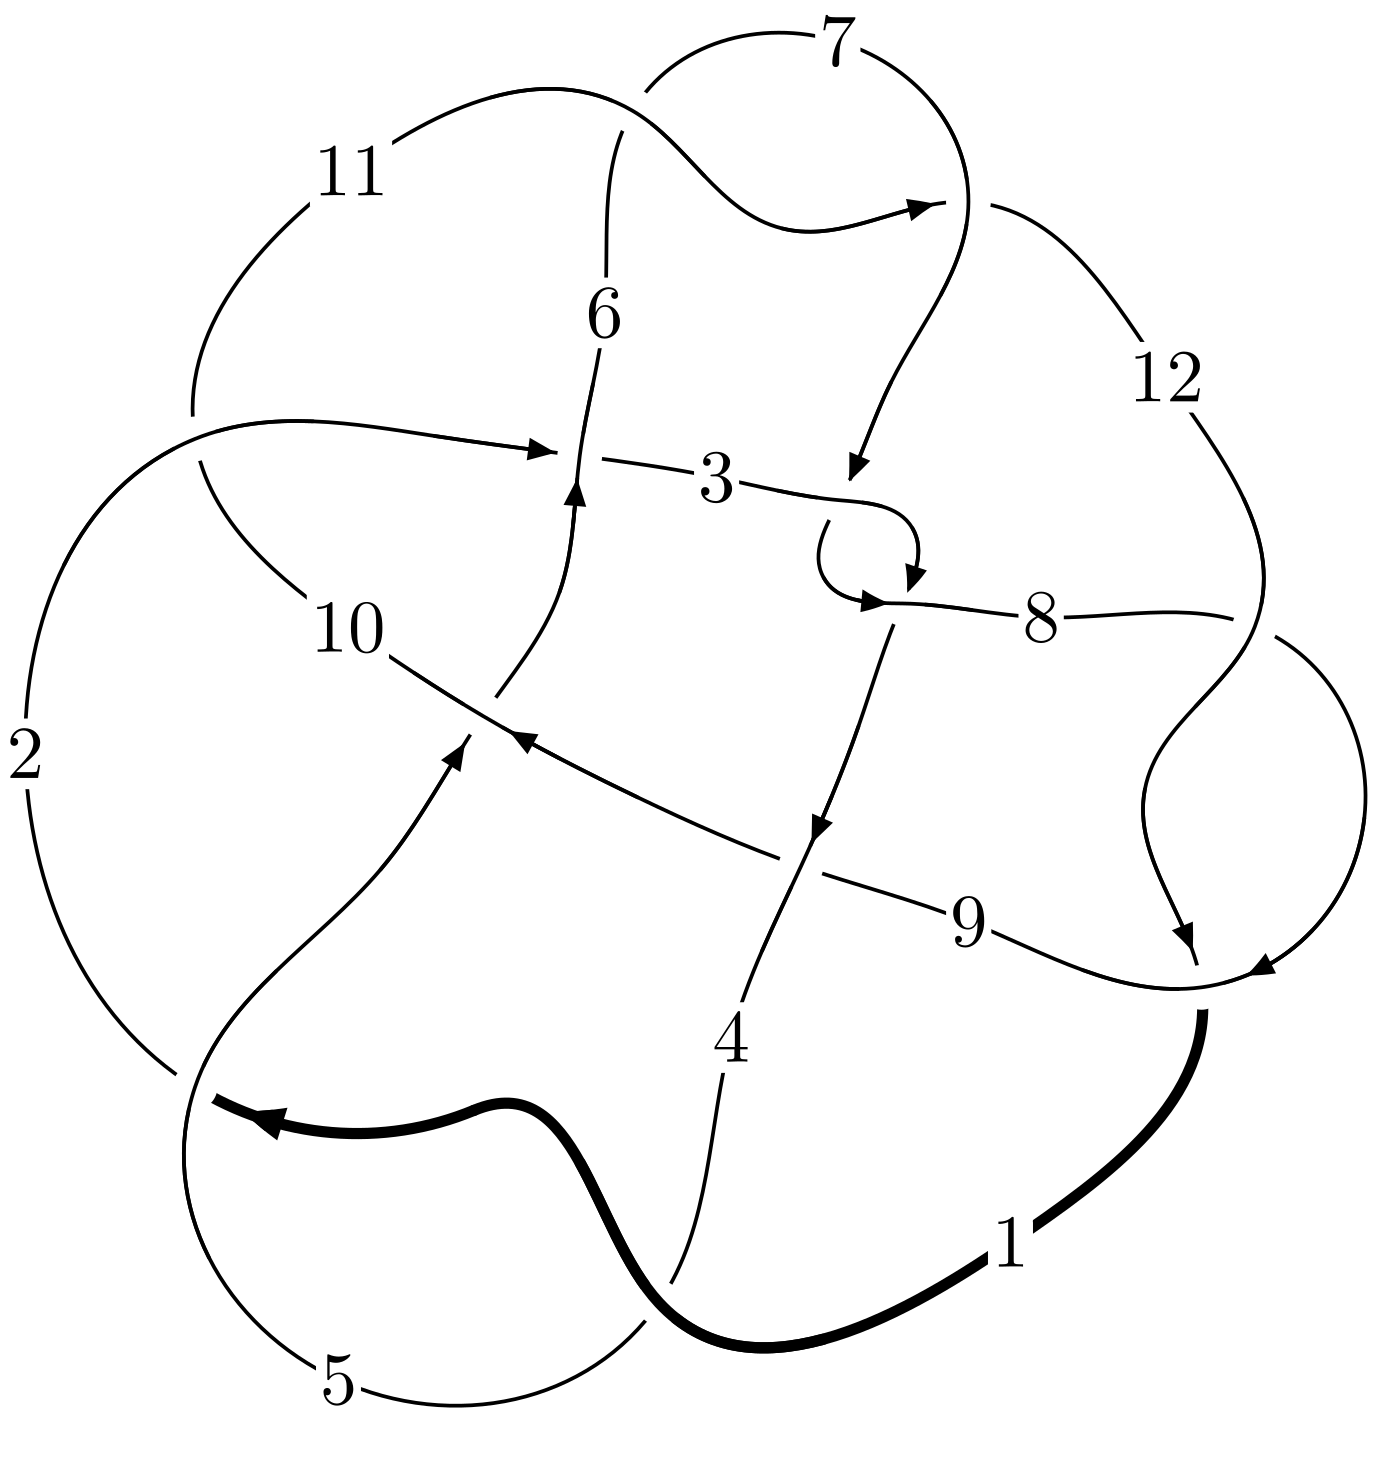
\includegraphics[width=112pt]{../../../GIT/diagram.site/Diagrams/png/2031_12a_1230.png}\\
\ \ \ A knot diagram\footnotemark}&
\allowdisplaybreaks
\textbf{Linearized knot diagam} \\
\cline{2-2}
 &
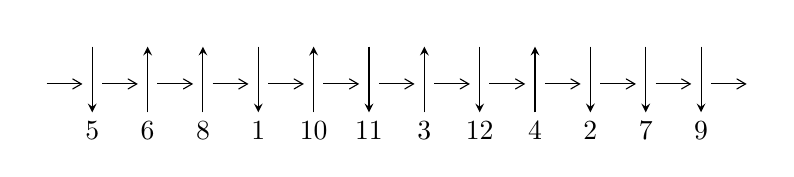
\begin{tikzpicture}[x=20pt, y=17pt]
	% nodes
	\node (C0) at (0, 0) {};
	\node (C1) at (1, 0) {};
	\node (C1U) at (1, +1) {};
	\node (C1D) at (1, -1) {5};

	\node (C2) at (2, 0) {};
	\node (C2U) at (2, +1) {};
	\node (C2D) at (2, -1) {6};

	\node (C3) at (3, 0) {};
	\node (C3U) at (3, +1) {};
	\node (C3D) at (3, -1) {8};

	\node (C4) at (4, 0) {};
	\node (C4U) at (4, +1) {};
	\node (C4D) at (4, -1) {1};

	\node (C5) at (5, 0) {};
	\node (C5U) at (5, +1) {};
	\node (C5D) at (5, -1) {10};

	\node (C6) at (6, 0) {};
	\node (C6U) at (6, +1) {};
	\node (C6D) at (6, -1) {11};

	\node (C7) at (7, 0) {};
	\node (C7U) at (7, +1) {};
	\node (C7D) at (7, -1) {3};

	\node (C8) at (8, 0) {};
	\node (C8U) at (8, +1) {};
	\node (C8D) at (8, -1) {12};

	\node (C9) at (9, 0) {};
	\node (C9U) at (9, +1) {};
	\node (C9D) at (9, -1) {4};

	\node (C10) at (10, 0) {};
	\node (C10U) at (10, +1) {};
	\node (C10D) at (10, -1) {2};

	\node (C11) at (11, 0) {};
	\node (C11U) at (11, +1) {};
	\node (C11D) at (11, -1) {7};

	\node (C12) at (12, 0) {};
	\node (C12U) at (12, +1) {};
	\node (C12D) at (12, -1) {9};
	\node (C13) at (13, 0) {};

	% arrows
	\draw[->,>={angle 60}]
	(C0) edge (C1) (C1) edge (C2) (C2) edge (C3) (C3) edge (C4) (C4) edge (C5) (C5) edge (C6) (C6) edge (C7) (C7) edge (C8) (C8) edge (C9) (C9) edge (C10) (C10) edge (C11) (C11) edge (C12) (C12) edge (C13) ;	\draw[->,>=stealth]
	(C1U) edge (C1D) (C2D) edge (C2U) (C3D) edge (C3U) (C4U) edge (C4D) (C5D) edge (C5U) (C6U) edge (C6D) (C7D) edge (C7U) (C8U) edge (C8D) (C9D) edge (C9U) (C10U) edge (C10D) (C11U) edge (C11D) (C12U) edge (C12D) ;
	\end{tikzpicture} \\
\hhline{~~} \\& 
\textbf{Solving Sequence} \\ \cline{2-2} 
 &
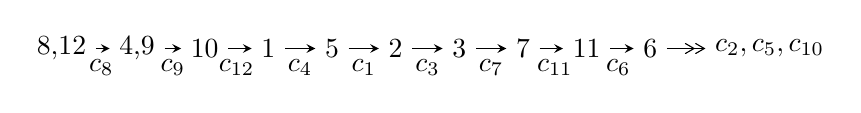
\begin{tikzpicture}[x=23pt, y=7pt]
	% node
	\node (A0) at (-1/8, 0) {8,12};
	\node (A1) at (17/16, 0) {4,9};
	\node (A2) at (17/8, 0) {10};
	\node (A3) at (25/8, 0) {1};
	\node (A4) at (33/8, 0) {5};
	\node (A5) at (41/8, 0) {2};
	\node (A6) at (49/8, 0) {3};
	\node (A7) at (57/8, 0) {7};
	\node (A8) at (65/8, 0) {11};
	\node (A9) at (73/8, 0) {6};
	\node (C1) at (1/2, -1) {$c_{8}$};
	\node (C2) at (13/8, -1) {$c_{9}$};
	\node (C3) at (21/8, -1) {$c_{12}$};
	\node (C4) at (29/8, -1) {$c_{4}$};
	\node (C5) at (37/8, -1) {$c_{1}$};
	\node (C6) at (45/8, -1) {$c_{3}$};
	\node (C7) at (53/8, -1) {$c_{7}$};
	\node (C8) at (61/8, -1) {$c_{11}$};
	\node (C9) at (69/8, -1) {$c_{6}$};
	\node (A10) at (11, 0) {$c_{2},c_{5},c_{10}$};

	% edge
	\draw[->,>=stealth]	
	(A0) edge (A1) (A1) edge (A2) (A2) edge (A3) (A3) edge (A4) (A4) edge (A5) (A5) edge (A6) (A6) edge (A7) (A7) edge (A8) (A8) edge (A9) ;
	\draw[->>,>={angle 60}]	
	(A9) edge (A10);
\end{tikzpicture} \\ 

\end{tabular} \\

\footnotetext{
The image of knot diagram is generated by the software ``\textbf{Draw programme}" developed by Andrew Bartholomew(\url{http://www.layer8.co.uk/maths/draw/index.htm\#Running-draw}), where we modified some parts for our purpose(\url{https://github.com/CATsTAILs/LinksPainter}).
}\phantom \\ \newline 
\centering \textbf{Ideals for irreducible components\footnotemark of $X_{\text{par}}$} 
 
\begin{align*}
I^u_{1}&=\langle 
-1.47607\times10^{645} u^{123}-7.69890\times10^{645} u^{122}+\cdots+2.13415\times10^{646} b-7.51217\times10^{648},\\
\phantom{I^u_{1}}&\phantom{= \langle  }1.94953\times10^{649} u^{123}+1.89460\times10^{649} u^{122}+\cdots+3.75397\times10^{649} a-2.18741\times10^{652},\\
\phantom{I^u_{1}}&\phantom{= \langle  }3 u^{124}+u^{123}+\cdots-11348 u+1759\rangle \\
I^u_{2}&=\langle 
-8331351990 u^{16}-18113236103 u^{15}+\cdots+1741200047 b-861824796,\\
\phantom{I^u_{2}}&\phantom{= \langle  }-11475305931 u^{16}-25118430940 u^{15}+\cdots+1741200047 a+6459102451,\\
\phantom{I^u_{2}}&\phantom{= \langle  }3 u^{17}+4 u^{16}+\cdots-16 u-1\rangle \\
\\
\end{align*}
\raggedright * 2 irreducible components of $\dim_{\mathbb{C}}=0$, with total 141 representations.\\
\footnotetext{All coefficients of polynomials are rational numbers. But the coefficients are sometimes approximated in decimal forms when there is not enough margin.}
\newpage
\renewcommand{\arraystretch}{1}
\centering \section*{I. $I^u_{1}= \langle -1.48\times10^{645} u^{123}-7.70\times10^{645} u^{122}+\cdots+2.13\times10^{646} b-7.51\times10^{648},\;1.95\times10^{649} u^{123}+1.89\times10^{649} u^{122}+\cdots+3.75\times10^{649} a-2.19\times10^{652},\;3 u^{124}+u^{123}+\cdots-11348 u+1759 \rangle$}
\flushleft \textbf{(i) Arc colorings}\\
\begin{tabular}{m{7pt} m{180pt} m{7pt} m{180pt} }
\flushright $a_{8}=$&$\begin{pmatrix}1\\0\end{pmatrix}$ \\
\flushright $a_{12}=$&$\begin{pmatrix}0\\u\end{pmatrix}$ \\
\flushright $a_{4}=$&$\begin{pmatrix}-0.519325 u^{123}-0.504692 u^{122}+\cdots-2320.34 u+582.693\\0.0691645 u^{123}+0.360748 u^{122}+\cdots-849.222 u+351.998\end{pmatrix}$ \\
\flushright $a_{9}=$&$\begin{pmatrix}1\\u^2\end{pmatrix}$ \\
\flushright $a_{10}=$&$\begin{pmatrix}-0.407021 u^{123}-0.999868 u^{122}+\cdots+537.930 u-374.222\\0.899250 u^{123}+1.15434 u^{122}+\cdots+3157.35 u-628.014\end{pmatrix}$ \\
\flushright $a_{1}=$&$\begin{pmatrix}- u\\- u^3+u\end{pmatrix}$ \\
\flushright $a_{5}=$&$\begin{pmatrix}-0.896202 u^{123}-1.09657 u^{122}+\cdots-3213.36 u+703.992\\-0.0927943 u^{123}+0.173284 u^{122}+\cdots-1498.89 u+504.077\end{pmatrix}$ \\
\flushright $a_{2}=$&$\begin{pmatrix}-0.546877 u^{123}-0.978883 u^{122}+\cdots-664.844 u-121.293\\0.178286 u^{123}-0.0195075 u^{122}+\cdots+1646.99 u-487.848\end{pmatrix}$ \\
\flushright $a_{3}=$&$\begin{pmatrix}-0.588490 u^{123}-0.865440 u^{122}+\cdots-1471.12 u+230.695\\0.0691645 u^{123}+0.360748 u^{122}+\cdots-849.222 u+351.998\end{pmatrix}$ \\
\flushright $a_{7}=$&$\begin{pmatrix}0.202534 u^{123}+0.558045 u^{122}+\cdots-629.192 u+344.874\\0.153383 u^{123}+0.399035 u^{122}+\cdots-194.488 u+136.408\end{pmatrix}$ \\
\flushright $a_{11}=$&$\begin{pmatrix}-1.48094 u^{123}-1.79696 u^{122}+\cdots-5580.55 u+1310.33\\-0.195990 u^{123}+0.0340962 u^{122}+\cdots-1997.47 u+649.189\end{pmatrix}$ \\
\flushright $a_{6}=$&$\begin{pmatrix}-0.878962 u^{123}-1.41971 u^{122}+\cdots-1890.44 u+315.400\\1.49342 u^{123}+1.99627 u^{122}+\cdots+4994.05 u-1026.70\end{pmatrix}$\\&\end{tabular}
\flushleft \textbf{(ii) Obstruction class $= -1$}\\~\\
\flushleft \textbf{(iii) Cusp Shapes $= -11.7889 u^{123}-14.0298 u^{122}+\cdots-44815.7 u+9573.22$}\\~\\
\newpage\renewcommand{\arraystretch}{1}
\flushleft \textbf{(iv) u-Polynomials at the component}\newline \\
\begin{tabular}{m{50pt}|m{274pt}}
Crossings & \hspace{64pt}u-Polynomials at each crossing \\
\hline $$\begin{aligned}c_{1},c_{4}\end{aligned}$$&$\begin{aligned}
&u^{124}+3 u^{123}+\cdots+44 u+4
\end{aligned}$\\
\hline $$\begin{aligned}c_{2}\end{aligned}$$&$\begin{aligned}
&3(3 u^{124}-7 u^{123}+\cdots-30 u-1)
\end{aligned}$\\
\hline $$\begin{aligned}c_{3},c_{7}\end{aligned}$$&$\begin{aligned}
&u^{124}+2 u^{123}+\cdots+6 u+1
\end{aligned}$\\
\hline $$\begin{aligned}c_{5}\end{aligned}$$&$\begin{aligned}
&3(3 u^{124}+13 u^{123}+\cdots+1185 u+161)
\end{aligned}$\\
\hline $$\begin{aligned}c_{6},c_{11}\end{aligned}$$&$\begin{aligned}
&u^{124}-45 u^{122}+\cdots-513 u-31
\end{aligned}$\\
\hline $$\begin{aligned}c_{8},c_{12}\end{aligned}$$&$\begin{aligned}
&3(3 u^{124}- u^{123}+\cdots+11348 u+1759)
\end{aligned}$\\
\hline $$\begin{aligned}c_{9}\end{aligned}$$&$\begin{aligned}
&u^{124}- u^{123}+\cdots-1188544 u-211971
\end{aligned}$\\
\hline $$\begin{aligned}c_{10}\end{aligned}$$&$\begin{aligned}
&u^{124}+2 u^{123}+\cdots-48068 u-4247
\end{aligned}$\\
\hline
\end{tabular}\\~\\
\newpage\renewcommand{\arraystretch}{1}
\flushleft \textbf{(v) Riley Polynomials at the component}\newline \\
\begin{tabular}{m{50pt}|m{274pt}}
Crossings & \hspace{64pt}Riley Polynomials at each crossing \\
\hline $$\begin{aligned}c_{1},c_{4}\end{aligned}$$&$\begin{aligned}
&y^{124}-97 y^{123}+\cdots+544 y+16
\end{aligned}$\\
\hline $$\begin{aligned}c_{2}\end{aligned}$$&$\begin{aligned}
&9(9 y^{124}-235 y^{123}+\cdots-228 y+1)
\end{aligned}$\\
\hline $$\begin{aligned}c_{3},c_{7}\end{aligned}$$&$\begin{aligned}
&y^{124}-66 y^{123}+\cdots-200 y+1
\end{aligned}$\\
\hline $$\begin{aligned}c_{5}\end{aligned}$$&$\begin{aligned}
&9(9 y^{124}-235 y^{123}+\cdots+463375 y+25921)
\end{aligned}$\\
\hline $$\begin{aligned}c_{6},c_{11}\end{aligned}$$&$\begin{aligned}
&y^{124}-90 y^{123}+\cdots-403847 y+961
\end{aligned}$\\
\hline $$\begin{aligned}c_{8},c_{12}\end{aligned}$$&$\begin{aligned}
&9(9 y^{124}-1087 y^{123}+\cdots-2.08080\times10^{8} y+3094081)
\end{aligned}$\\
\hline $$\begin{aligned}c_{9}\end{aligned}$$&$\begin{aligned}
&y^{124}+29 y^{123}+\cdots+896206404524 y+44931704841
\end{aligned}$\\
\hline $$\begin{aligned}c_{10}\end{aligned}$$&$\begin{aligned}
&y^{124}-44 y^{123}+\cdots-1625831284 y+18037009
\end{aligned}$\\
\hline
\end{tabular}\\~\\
\newpage\flushleft \textbf{(vi) Complex Volumes and Cusp Shapes}
$$\begin{array}{c|c|c}  
\text{Solutions to }I^u_{1}& \I (\text{vol} + \sqrt{-1}CS) & \text{Cusp shape}\\
 \hline 
\begin{aligned}
u &= \phantom{-}0.788605 + 0.603204 I \\
a &= -0.773510 + 0.152551 I \\
b &= -1.155560 - 0.574558 I\end{aligned}
 & -2.43728 + 1.83748 I & \phantom{-0.000000 } 0 \\ \hline\begin{aligned}
u &= \phantom{-}0.788605 - 0.603204 I \\
a &= -0.773510 - 0.152551 I \\
b &= -1.155560 + 0.574558 I\end{aligned}
 & -2.43728 - 1.83748 I & \phantom{-0.000000 } 0 \\ \hline\begin{aligned}
u &= \phantom{-}0.123262 + 1.005660 I \\
a &= \phantom{-}0.311877 + 0.261104 I \\
b &= -1.165100 + 0.482298 I\end{aligned}
 & \phantom{-}1.31303 - 5.91813 I & \phantom{-0.000000 } 0 \\ \hline\begin{aligned}
u &= \phantom{-}0.123262 - 1.005660 I \\
a &= \phantom{-}0.311877 - 0.261104 I \\
b &= -1.165100 - 0.482298 I\end{aligned}
 & \phantom{-}1.31303 + 5.91813 I & \phantom{-0.000000 } 0 \\ \hline\begin{aligned}
u &= -0.949710 + 0.238781 I \\
a &= \phantom{-}0.58259 + 1.35786 I \\
b &= \phantom{-}1.171990 + 0.531039 I\end{aligned}
 & \phantom{-}1.34709 + 1.96348 I & \phantom{-0.000000 } 0 \\ \hline\begin{aligned}
u &= -0.949710 - 0.238781 I \\
a &= \phantom{-}0.58259 - 1.35786 I \\
b &= \phantom{-}1.171990 - 0.531039 I\end{aligned}
 & \phantom{-}1.34709 - 1.96348 I & \phantom{-0.000000 } 0 \\ \hline\begin{aligned}
u &= -0.975980 + 0.302633 I \\
a &= -0.08994 + 1.56774 I \\
b &= \phantom{-}0.342586 + 0.781780 I\end{aligned}
 & -0.96971 + 3.60554 I & \phantom{-0.000000 } 0 \\ \hline\begin{aligned}
u &= -0.975980 - 0.302633 I \\
a &= -0.08994 - 1.56774 I \\
b &= \phantom{-}0.342586 - 0.781780 I\end{aligned}
 & -0.96971 - 3.60554 I & \phantom{-0.000000 } 0 \\ \hline\begin{aligned}
u &= \phantom{-}0.968093 + 0.072187 I \\
a &= -2.42423 - 2.56791 I \\
b &= -0.876990 - 0.089373 I\end{aligned}
 & -4.80410 - 0.11389 I & \phantom{-0.000000 } 0 \\ \hline\begin{aligned}
u &= \phantom{-}0.968093 - 0.072187 I \\
a &= -2.42423 + 2.56791 I \\
b &= -0.876990 + 0.089373 I\end{aligned}
 & -4.80410 + 0.11389 I & \phantom{-0.000000 } 0\\
 \hline 
 \end{array}$$\newpage$$\begin{array}{c|c|c}  
\text{Solutions to }I^u_{1}& \I (\text{vol} + \sqrt{-1}CS) & \text{Cusp shape}\\
 \hline 
\begin{aligned}
u &= \phantom{-}1.05831\phantom{ +0.000000I} \\
a &= \phantom{-}1.48125\phantom{ +0.000000I} \\
b &= -1.29432\phantom{ +0.000000I}\end{aligned}
 & -5.24214\phantom{ +0.000000I} & \phantom{-0.000000 } 0 \\ \hline\begin{aligned}
u &= \phantom{-}0.894123 + 0.279210 I \\
a &= -0.10822 + 2.16309 I \\
b &= -1.16089 + 1.18171 I\end{aligned}
 & -2.48013 - 5.46707 I & \phantom{-0.000000 } 0 \\ \hline\begin{aligned}
u &= \phantom{-}0.894123 - 0.279210 I \\
a &= -0.10822 - 2.16309 I \\
b &= -1.16089 - 1.18171 I\end{aligned}
 & -2.48013 + 5.46707 I & \phantom{-0.000000 } 0 \\ \hline\begin{aligned}
u &= -0.979983 + 0.431569 I \\
a &= \phantom{-}0.575071 - 1.253460 I \\
b &= \phantom{-}0.147458 - 0.031198 I\end{aligned}
 & -5.89109 + 9.09334 I & \phantom{-0.000000 } 0 \\ \hline\begin{aligned}
u &= -0.979983 - 0.431569 I \\
a &= \phantom{-}0.575071 + 1.253460 I \\
b &= \phantom{-}0.147458 + 0.031198 I\end{aligned}
 & -5.89109 - 9.09334 I & \phantom{-0.000000 } 0 \\ \hline\begin{aligned}
u &= \phantom{-}0.903842 + 0.580723 I \\
a &= -0.856001 - 0.351840 I \\
b &= -0.153008 - 0.040285 I\end{aligned}
 & -5.25838 - 0.22234 I & \phantom{-0.000000 } 0 \\ \hline\begin{aligned}
u &= \phantom{-}0.903842 - 0.580723 I \\
a &= -0.856001 + 0.351840 I \\
b &= -0.153008 + 0.040285 I\end{aligned}
 & -5.25838 + 0.22234 I & \phantom{-0.000000 } 0 \\ \hline\begin{aligned}
u &= \phantom{-}0.888925 + 0.236273 I \\
a &= -0.75252 - 1.70671 I \\
b &= \phantom{-}1.045960 - 0.225775 I\end{aligned}
 & \phantom{-}0.344321 - 0.915316 I & \phantom{-0.000000 } 0 \\ \hline\begin{aligned}
u &= \phantom{-}0.888925 - 0.236273 I \\
a &= -0.75252 + 1.70671 I \\
b &= \phantom{-}1.045960 + 0.225775 I\end{aligned}
 & \phantom{-}0.344321 + 0.915316 I & \phantom{-0.000000 } 0 \\ \hline\begin{aligned}
u &= \phantom{-}0.086900 + 1.088350 I \\
a &= -0.338466 - 0.485239 I \\
b &= \phantom{-}1.248980 - 0.176372 I\end{aligned}
 & \phantom{-}2.07576 - 6.77659 I & \phantom{-0.000000 } 0\\
 \hline 
 \end{array}$$\newpage$$\begin{array}{c|c|c}  
\text{Solutions to }I^u_{1}& \I (\text{vol} + \sqrt{-1}CS) & \text{Cusp shape}\\
 \hline 
\begin{aligned}
u &= \phantom{-}0.086900 - 1.088350 I \\
a &= -0.338466 + 0.485239 I \\
b &= \phantom{-}1.248980 + 0.176372 I\end{aligned}
 & \phantom{-}2.07576 + 6.77659 I & \phantom{-0.000000 } 0 \\ \hline\begin{aligned}
u &= -0.133340 + 0.893430 I \\
a &= \phantom{-}0.255453 + 0.028036 I \\
b &= -1.290390 + 0.097289 I\end{aligned}
 & \phantom{-}6.38240 - 2.65405 I & \phantom{-0.000000 } 0 \\ \hline\begin{aligned}
u &= -0.133340 - 0.893430 I \\
a &= \phantom{-}0.255453 - 0.028036 I \\
b &= -1.290390 - 0.097289 I\end{aligned}
 & \phantom{-}6.38240 + 2.65405 I & \phantom{-0.000000 } 0 \\ \hline\begin{aligned}
u &= \phantom{-}1.103370 + 0.111328 I \\
a &= -0.00971 + 2.27977 I \\
b &= \phantom{-}0.459954 + 0.548916 I\end{aligned}
 & -3.75488 - 0.79756 I & \phantom{-0.000000 } 0 \\ \hline\begin{aligned}
u &= \phantom{-}1.103370 - 0.111328 I \\
a &= -0.00971 - 2.27977 I \\
b &= \phantom{-}0.459954 - 0.548916 I\end{aligned}
 & -3.75488 + 0.79756 I & \phantom{-0.000000 } 0 \\ \hline\begin{aligned}
u &= \phantom{-}1.094220 + 0.218141 I \\
a &= \phantom{-}0.86694 - 1.59283 I \\
b &= \phantom{-}0.807249 - 0.142085 I\end{aligned}
 & -0.612185 - 0.724132 I & \phantom{-0.000000 } 0 \\ \hline\begin{aligned}
u &= \phantom{-}1.094220 - 0.218141 I \\
a &= \phantom{-}0.86694 + 1.59283 I \\
b &= \phantom{-}0.807249 + 0.142085 I\end{aligned}
 & -0.612185 + 0.724132 I & \phantom{-0.000000 } 0 \\ \hline\begin{aligned}
u &= \phantom{-}0.157240 + 1.110290 I \\
a &= -0.110324 - 0.166987 I \\
b &= \phantom{-}1.169760 + 0.436291 I\end{aligned}
 & \phantom{-}1.84863 + 7.63093 I & \phantom{-0.000000 } 0 \\ \hline\begin{aligned}
u &= \phantom{-}0.157240 - 1.110290 I \\
a &= -0.110324 + 0.166987 I \\
b &= \phantom{-}1.169760 - 0.436291 I\end{aligned}
 & \phantom{-}1.84863 - 7.63093 I & \phantom{-0.000000 } 0 \\ \hline\begin{aligned}
u &= \phantom{-}0.834550 + 0.268312 I \\
a &= \phantom{-}0.553460 + 0.612766 I \\
b &= -0.371624 + 0.067577 I\end{aligned}
 & -1.40266 - 0.46426 I & \phantom{-0.000000 } 0\\
 \hline 
 \end{array}$$\newpage$$\begin{array}{c|c|c}  
\text{Solutions to }I^u_{1}& \I (\text{vol} + \sqrt{-1}CS) & \text{Cusp shape}\\
 \hline 
\begin{aligned}
u &= \phantom{-}0.834550 - 0.268312 I \\
a &= \phantom{-}0.553460 - 0.612766 I \\
b &= -0.371624 - 0.067577 I\end{aligned}
 & -1.40266 + 0.46426 I & \phantom{-0.000000 } 0 \\ \hline\begin{aligned}
u &= \phantom{-}1.138310 + 0.017075 I \\
a &= \phantom{-}0.91942 - 1.70196 I \\
b &= \phantom{-}1.69305 - 1.17482 I\end{aligned}
 & -6.39003 + 3.25066 I & \phantom{-0.000000 } 0 \\ \hline\begin{aligned}
u &= \phantom{-}1.138310 - 0.017075 I \\
a &= \phantom{-}0.91942 + 1.70196 I \\
b &= \phantom{-}1.69305 + 1.17482 I\end{aligned}
 & -6.39003 - 3.25066 I & \phantom{-0.000000 } 0 \\ \hline\begin{aligned}
u &= \phantom{-}1.142860 + 0.128567 I \\
a &= \phantom{-}0.22185 + 1.75605 I \\
b &= \phantom{-}0.19599 + 1.80667 I\end{aligned}
 & -5.17825 - 5.30127 I & \phantom{-0.000000 } 0 \\ \hline\begin{aligned}
u &= \phantom{-}1.142860 - 0.128567 I \\
a &= \phantom{-}0.22185 - 1.75605 I \\
b &= \phantom{-}0.19599 - 1.80667 I\end{aligned}
 & -5.17825 + 5.30127 I & \phantom{-0.000000 } 0 \\ \hline\begin{aligned}
u &= -1.158250 + 0.020836 I \\
a &= -0.08583 + 1.87683 I \\
b &= \phantom{-}1.161920 + 0.643909 I\end{aligned}
 & -8.02058 + 8.45569 I & \phantom{-0.000000 } 0 \\ \hline\begin{aligned}
u &= -1.158250 - 0.020836 I \\
a &= -0.08583 - 1.87683 I \\
b &= \phantom{-}1.161920 - 0.643909 I\end{aligned}
 & -8.02058 - 8.45569 I & \phantom{-0.000000 } 0 \\ \hline\begin{aligned}
u &= \phantom{-}1.15977\phantom{ +0.000000I} \\
a &= -1.40356\phantom{ +0.000000I} \\
b &= \phantom{-}0.492111\phantom{ +0.000000I}\end{aligned}
 & -3.85647\phantom{ +0.000000I} & \phantom{-0.000000 } 0 \\ \hline\begin{aligned}
u &= \phantom{-}0.530974 + 0.632952 I \\
a &= \phantom{-}0.224564 + 0.305269 I \\
b &= -0.608186 - 0.414278 I\end{aligned}
 & -1.54550 - 0.57882 I & \phantom{-0.000000 } 0 \\ \hline\begin{aligned}
u &= \phantom{-}0.530974 - 0.632952 I \\
a &= \phantom{-}0.224564 - 0.305269 I \\
b &= -0.608186 + 0.414278 I\end{aligned}
 & -1.54550 + 0.57882 I & \phantom{-0.000000 } 0\\
 \hline 
 \end{array}$$\newpage$$\begin{array}{c|c|c}  
\text{Solutions to }I^u_{1}& \I (\text{vol} + \sqrt{-1}CS) & \text{Cusp shape}\\
 \hline 
\begin{aligned}
u &= -1.175520 + 0.046030 I \\
a &= \phantom{-}0.057140 - 1.114490 I \\
b &= -1.292650 - 0.499292 I\end{aligned}
 & -8.20014 + 1.57315 I & \phantom{-0.000000 } 0 \\ \hline\begin{aligned}
u &= -1.175520 - 0.046030 I \\
a &= \phantom{-}0.057140 + 1.114490 I \\
b &= -1.292650 + 0.499292 I\end{aligned}
 & -8.20014 - 1.57315 I & \phantom{-0.000000 } 0 \\ \hline\begin{aligned}
u &= \phantom{-}0.036239 + 0.811904 I \\
a &= -0.126186 + 0.584919 I \\
b &= -0.247828 + 0.521765 I\end{aligned}
 & -2.49622 - 4.31640 I & \phantom{-0.000000 } 0 \\ \hline\begin{aligned}
u &= \phantom{-}0.036239 - 0.811904 I \\
a &= -0.126186 - 0.584919 I \\
b &= -0.247828 - 0.521765 I\end{aligned}
 & -2.49622 + 4.31640 I & \phantom{-0.000000 } 0 \\ \hline\begin{aligned}
u &= -1.168590 + 0.220171 I \\
a &= -0.550977 + 1.260230 I \\
b &= -0.796498 + 0.896199 I\end{aligned}
 & -5.33472 + 3.61289 I & \phantom{-0.000000 } 0 \\ \hline\begin{aligned}
u &= -1.168590 - 0.220171 I \\
a &= -0.550977 - 1.260230 I \\
b &= -0.796498 - 0.896199 I\end{aligned}
 & -5.33472 - 3.61289 I & \phantom{-0.000000 } 0 \\ \hline\begin{aligned}
u &= \phantom{-}1.065910 + 0.535700 I \\
a &= \phantom{-}0.26281 + 1.46778 I \\
b &= -1.025860 + 0.788200 I\end{aligned}
 & -3.22218 - 4.36249 I & \phantom{-0.000000 } 0 \\ \hline\begin{aligned}
u &= \phantom{-}1.065910 - 0.535700 I \\
a &= \phantom{-}0.26281 - 1.46778 I \\
b &= -1.025860 - 0.788200 I\end{aligned}
 & -3.22218 + 4.36249 I & \phantom{-0.000000 } 0 \\ \hline\begin{aligned}
u &= -1.22576\phantom{ +0.000000I} \\
a &= -1.01823\phantom{ +0.000000I} \\
b &= -2.03524\phantom{ +0.000000I}\end{aligned}
 & -7.61392\phantom{ +0.000000I} & \phantom{-0.000000 } 0 \\ \hline\begin{aligned}
u &= -1.229930 + 0.175863 I \\
a &= -0.61442 + 1.59509 I \\
b &= -0.66953 + 1.49455 I\end{aligned}
 & -5.70033 + 3.64848 I & \phantom{-0.000000 } 0\\
 \hline 
 \end{array}$$\newpage$$\begin{array}{c|c|c}  
\text{Solutions to }I^u_{1}& \I (\text{vol} + \sqrt{-1}CS) & \text{Cusp shape}\\
 \hline 
\begin{aligned}
u &= -1.229930 - 0.175863 I \\
a &= -0.61442 - 1.59509 I \\
b &= -0.66953 - 1.49455 I\end{aligned}
 & -5.70033 - 3.64848 I & \phantom{-0.000000 } 0 \\ \hline\begin{aligned}
u &= -1.198130 + 0.360507 I \\
a &= \phantom{-}0.48307 + 1.57590 I \\
b &= \phantom{-}1.40506 + 0.91636 I\end{aligned}
 & -0.11264 + 5.91385 I & \phantom{-0.000000 } 0 \\ \hline\begin{aligned}
u &= -1.198130 - 0.360507 I \\
a &= \phantom{-}0.48307 - 1.57590 I \\
b &= \phantom{-}1.40506 - 0.91636 I\end{aligned}
 & -0.11264 - 5.91385 I & \phantom{-0.000000 } 0 \\ \hline\begin{aligned}
u &= -0.742890\phantom{ +0.000000I} \\
a &= \phantom{-}1.01419\phantom{ +0.000000I} \\
b &= \phantom{-}1.67101\phantom{ +0.000000I}\end{aligned}
 & \phantom{-}3.02186\phantom{ +0.000000I} & \phantom{-0.000000 } 0 \\ \hline\begin{aligned}
u &= -0.586348 + 0.441635 I \\
a &= -0.34504 + 1.62898 I \\
b &= \phantom{-}0.214066 - 0.203261 I\end{aligned}
 & -1.17179 + 4.15296 I & \phantom{-0.000000 } 0 \\ \hline\begin{aligned}
u &= -0.586348 - 0.441635 I \\
a &= -0.34504 - 1.62898 I \\
b &= \phantom{-}0.214066 + 0.203261 I\end{aligned}
 & -1.17179 - 4.15296 I & \phantom{-0.000000 } 0 \\ \hline\begin{aligned}
u &= -0.119121 + 0.708028 I \\
a &= -0.095345 + 0.505809 I \\
b &= \phantom{-}1.239320 - 0.380272 I\end{aligned}
 & \phantom{-}3.18902 - 1.94291 I & \phantom{-0.000000 } 0 \\ \hline\begin{aligned}
u &= -0.119121 - 0.708028 I \\
a &= -0.095345 - 0.505809 I \\
b &= \phantom{-}1.239320 + 0.380272 I\end{aligned}
 & \phantom{-}3.18902 + 1.94291 I & \phantom{-0.000000 } 0 \\ \hline\begin{aligned}
u &= -1.214530 + 0.410822 I \\
a &= \phantom{-}0.126987 - 1.371560 I \\
b &= -1.247480 - 0.603820 I\end{aligned}
 & -4.20839 + 8.51329 I & \phantom{-0.000000 } 0 \\ \hline\begin{aligned}
u &= -1.214530 - 0.410822 I \\
a &= \phantom{-}0.126987 + 1.371560 I \\
b &= -1.247480 + 0.603820 I\end{aligned}
 & -4.20839 - 8.51329 I & \phantom{-0.000000 } 0\\
 \hline 
 \end{array}$$\newpage$$\begin{array}{c|c|c}  
\text{Solutions to }I^u_{1}& \I (\text{vol} + \sqrt{-1}CS) & \text{Cusp shape}\\
 \hline 
\begin{aligned}
u &= \phantom{-}0.714154 + 1.074430 I \\
a &= \phantom{-}0.715561 + 0.192223 I \\
b &= -0.947446 + 0.161518 I\end{aligned}
 & -1.86971 - 2.12951 I & \phantom{-0.000000 } 0 \\ \hline\begin{aligned}
u &= \phantom{-}0.714154 - 1.074430 I \\
a &= \phantom{-}0.715561 - 0.192223 I \\
b &= -0.947446 - 0.161518 I\end{aligned}
 & -1.86971 + 2.12951 I & \phantom{-0.000000 } 0 \\ \hline\begin{aligned}
u &= \phantom{-}1.246760 + 0.376459 I \\
a &= -0.24354 + 1.80084 I \\
b &= -0.846234 + 0.323241 I\end{aligned}
 & -4.43600 - 2.51207 I & \phantom{-0.000000 } 0 \\ \hline\begin{aligned}
u &= \phantom{-}1.246760 - 0.376459 I \\
a &= -0.24354 - 1.80084 I \\
b &= -0.846234 - 0.323241 I\end{aligned}
 & -4.43600 + 2.51207 I & \phantom{-0.000000 } 0 \\ \hline\begin{aligned}
u &= -1.213930 + 0.481250 I \\
a &= -0.40166 - 1.36719 I \\
b &= -1.209900 - 0.435379 I\end{aligned}
 & \phantom{-}3.05232 + 7.60282 I & \phantom{-0.000000 } 0 \\ \hline\begin{aligned}
u &= -1.213930 - 0.481250 I \\
a &= -0.40166 + 1.36719 I \\
b &= -1.209900 + 0.435379 I\end{aligned}
 & \phantom{-}3.05232 - 7.60282 I & \phantom{-0.000000 } 0 \\ \hline\begin{aligned}
u &= -0.201782 + 0.659839 I \\
a &= -0.117132 + 0.905608 I \\
b &= \phantom{-}1.275610 + 0.109948 I\end{aligned}
 & \phantom{-}3.29232 + 1.21871 I & \phantom{-0.000000 } 0 \\ \hline\begin{aligned}
u &= -0.201782 - 0.659839 I \\
a &= -0.117132 - 0.905608 I \\
b &= \phantom{-}1.275610 - 0.109948 I\end{aligned}
 & \phantom{-}3.29232 - 1.21871 I & \phantom{-0.000000 } 0 \\ \hline\begin{aligned}
u &= \phantom{-}1.287490 + 0.327049 I \\
a &= -0.768832 + 1.012340 I \\
b &= -1.233210 + 0.380204 I\end{aligned}
 & \phantom{-}1.75057 - 1.55337 I & \phantom{-0.000000 } 0 \\ \hline\begin{aligned}
u &= \phantom{-}1.287490 - 0.327049 I \\
a &= -0.768832 - 1.012340 I \\
b &= -1.233210 - 0.380204 I\end{aligned}
 & \phantom{-}1.75057 + 1.55337 I & \phantom{-0.000000 } 0\\
 \hline 
 \end{array}$$\newpage$$\begin{array}{c|c|c}  
\text{Solutions to }I^u_{1}& \I (\text{vol} + \sqrt{-1}CS) & \text{Cusp shape}\\
 \hline 
\begin{aligned}
u &= -1.346130 + 0.093012 I \\
a &= -0.424411 + 1.038860 I \\
b &= -0.284819 + 0.998234 I\end{aligned}
 & -7.24521 + 2.71118 I & \phantom{-0.000000 } 0 \\ \hline\begin{aligned}
u &= -1.346130 - 0.093012 I \\
a &= -0.424411 - 1.038860 I \\
b &= -0.284819 - 0.998234 I\end{aligned}
 & -7.24521 - 2.71118 I & \phantom{-0.000000 } 0 \\ \hline\begin{aligned}
u &= \phantom{-}1.256950 + 0.549835 I \\
a &= \phantom{-}0.193727 - 1.393470 I \\
b &= \phantom{-}1.36822 - 0.77314 I\end{aligned}
 & -1.60499 - 13.40180 I & \phantom{-0.000000 } 0 \\ \hline\begin{aligned}
u &= \phantom{-}1.256950 - 0.549835 I \\
a &= \phantom{-}0.193727 + 1.393470 I \\
b &= \phantom{-}1.36822 + 0.77314 I\end{aligned}
 & -1.60499 + 13.40180 I & \phantom{-0.000000 } 0 \\ \hline\begin{aligned}
u &= -0.300969 + 1.340690 I \\
a &= \phantom{-}0.192114 - 0.208650 I \\
b &= -1.211350 - 0.431036 I\end{aligned}
 & -2.09713 + 12.66730 I & \phantom{-0.000000 } 0 \\ \hline\begin{aligned}
u &= -0.300969 - 1.340690 I \\
a &= \phantom{-}0.192114 + 0.208650 I \\
b &= -1.211350 + 0.431036 I\end{aligned}
 & -2.09713 - 12.66730 I & \phantom{-0.000000 } 0 \\ \hline\begin{aligned}
u &= -1.286800 + 0.525371 I \\
a &= \phantom{-}0.126633 - 1.213530 I \\
b &= -0.517404 - 0.556031 I\end{aligned}
 & -6.23413 + 9.08506 I & \phantom{-0.000000 } 0 \\ \hline\begin{aligned}
u &= -1.286800 - 0.525371 I \\
a &= \phantom{-}0.126633 + 1.213530 I \\
b &= -0.517404 + 0.556031 I\end{aligned}
 & -6.23413 - 9.08506 I & \phantom{-0.000000 } 0 \\ \hline\begin{aligned}
u &= -0.475834 + 0.374162 I \\
a &= \phantom{-}1.79148 - 0.41794 I \\
b &= \phantom{-}0.336927 + 0.600944 I\end{aligned}
 & -5.88107 + 8.91166 I & \phantom{-0.000000 } 0 \\ \hline\begin{aligned}
u &= -0.475834 - 0.374162 I \\
a &= \phantom{-}1.79148 + 0.41794 I \\
b &= \phantom{-}0.336927 - 0.600944 I\end{aligned}
 & -5.88107 - 8.91166 I & \phantom{-0.000000 } 0\\
 \hline 
 \end{array}$$\newpage$$\begin{array}{c|c|c}  
\text{Solutions to }I^u_{1}& \I (\text{vol} + \sqrt{-1}CS) & \text{Cusp shape}\\
 \hline 
\begin{aligned}
u &= \phantom{-}1.382080 + 0.284573 I \\
a &= -0.12556 - 1.44107 I \\
b &= -0.11274 - 1.42408 I\end{aligned}
 & -11.5203 - 11.9060 I & \phantom{-0.000000 } 0 \\ \hline\begin{aligned}
u &= \phantom{-}1.382080 - 0.284573 I \\
a &= -0.12556 + 1.44107 I \\
b &= -0.11274 + 1.42408 I\end{aligned}
 & -11.5203 + 11.9060 I & \phantom{-0.000000 } 0 \\ \hline\begin{aligned}
u &= \phantom{-}1.41099 + 0.32694 I \\
a &= \phantom{-}0.79167 - 1.36801 I \\
b &= \phantom{-}1.077230 - 0.477025 I\end{aligned}
 & -1.85313 - 4.94493 I & \phantom{-0.000000 } 0 \\ \hline\begin{aligned}
u &= \phantom{-}1.41099 - 0.32694 I \\
a &= \phantom{-}0.79167 + 1.36801 I \\
b &= \phantom{-}1.077230 + 0.477025 I\end{aligned}
 & -1.85313 + 4.94493 I & \phantom{-0.000000 } 0 \\ \hline\begin{aligned}
u &= \phantom{-}1.42016 + 0.30725 I \\
a &= \phantom{-}0.076634 + 1.023840 I \\
b &= \phantom{-}0.317383 + 1.056200 I\end{aligned}
 & -11.76120 - 3.73889 I & \phantom{-0.000000 } 0 \\ \hline\begin{aligned}
u &= \phantom{-}1.42016 - 0.30725 I \\
a &= \phantom{-}0.076634 - 1.023840 I \\
b &= \phantom{-}0.317383 - 1.056200 I\end{aligned}
 & -11.76120 + 3.73889 I & \phantom{-0.000000 } 0 \\ \hline\begin{aligned}
u &= -1.38533 + 0.45833 I \\
a &= -0.26988 - 1.54224 I \\
b &= -1.25913 - 0.77998 I\end{aligned}
 & -3.42270 + 11.12110 I & \phantom{-0.000000 } 0 \\ \hline\begin{aligned}
u &= -1.38533 - 0.45833 I \\
a &= -0.26988 + 1.54224 I \\
b &= -1.25913 + 0.77998 I\end{aligned}
 & -3.42270 - 11.12110 I & \phantom{-0.000000 } 0 \\ \hline\begin{aligned}
u &= -0.336986 + 0.414236 I \\
a &= \phantom{-}1.13438 - 1.71290 I \\
b &= -0.674367 + 0.429281 I\end{aligned}
 & -1.42144 - 4.58216 I & -3.65378 + 4.57244 I \\ \hline\begin{aligned}
u &= -0.336986 - 0.414236 I \\
a &= \phantom{-}1.13438 + 1.71290 I \\
b &= -0.674367 - 0.429281 I\end{aligned}
 & -1.42144 + 4.58216 I & -3.65378 - 4.57244 I\\
 \hline 
 \end{array}$$\newpage$$\begin{array}{c|c|c}  
\text{Solutions to }I^u_{1}& \I (\text{vol} + \sqrt{-1}CS) & \text{Cusp shape}\\
 \hline 
\begin{aligned}
u &= -1.38917 + 0.49444 I \\
a &= \phantom{-}0.34978 + 1.43405 I \\
b &= \phantom{-}1.191080 + 0.416776 I\end{aligned}
 & -2.56414 + 12.34190 I & \phantom{-0.000000 } 0 \\ \hline\begin{aligned}
u &= -1.38917 - 0.49444 I \\
a &= \phantom{-}0.34978 - 1.43405 I \\
b &= \phantom{-}1.191080 - 0.416776 I\end{aligned}
 & -2.56414 - 12.34190 I & \phantom{-0.000000 } 0 \\ \hline\begin{aligned}
u &= -1.46872 + 0.13574 I \\
a &= \phantom{-}0.710171 + 1.157920 I \\
b &= \phantom{-}0.441897 + 0.950718 I\end{aligned}
 & -10.28200 - 2.62507 I & \phantom{-0.000000 } 0 \\ \hline\begin{aligned}
u &= -1.46872 - 0.13574 I \\
a &= \phantom{-}0.710171 - 1.157920 I \\
b &= \phantom{-}0.441897 - 0.950718 I\end{aligned}
 & -10.28200 + 2.62507 I & \phantom{-0.000000 } 0 \\ \hline\begin{aligned}
u &= -1.25214 + 0.79663 I \\
a &= -0.186292 + 0.406134 I \\
b &= \phantom{-}1.163230 + 0.325120 I\end{aligned}
 & -2.21685 + 0.93511 I & \phantom{-0.000000 } 0 \\ \hline\begin{aligned}
u &= -1.25214 - 0.79663 I \\
a &= -0.186292 - 0.406134 I \\
b &= \phantom{-}1.163230 - 0.325120 I\end{aligned}
 & -2.21685 - 0.93511 I & \phantom{-0.000000 } 0 \\ \hline\begin{aligned}
u &= -1.46287 + 0.28250 I \\
a &= \phantom{-}0.029871 - 1.060580 I \\
b &= \phantom{-}0.062869 - 1.043970 I\end{aligned}
 & -12.53470 + 3.74102 I & \phantom{-0.000000 } 0 \\ \hline\begin{aligned}
u &= -1.46287 - 0.28250 I \\
a &= \phantom{-}0.029871 + 1.060580 I \\
b &= \phantom{-}0.062869 + 1.043970 I\end{aligned}
 & -12.53470 - 3.74102 I & \phantom{-0.000000 } 0 \\ \hline\begin{aligned}
u &= \phantom{-}0.187016 + 0.472108 I \\
a &= \phantom{-}1.135900 - 0.469578 I \\
b &= -0.222276 - 0.738246 I\end{aligned}
 & -1.55739 - 1.34736 I & \phantom{-0.000000 -}0. + 3.86805 I \\ \hline\begin{aligned}
u &= \phantom{-}0.187016 - 0.472108 I \\
a &= \phantom{-}1.135900 + 0.469578 I \\
b &= -0.222276 + 0.738246 I\end{aligned}
 & -1.55739 + 1.34736 I & \phantom{-0.000000 } 0. - 3.86805 I\\
 \hline 
 \end{array}$$\newpage$$\begin{array}{c|c|c}  
\text{Solutions to }I^u_{1}& \I (\text{vol} + \sqrt{-1}CS) & \text{Cusp shape}\\
 \hline 
\begin{aligned}
u &= \phantom{-}1.54306\phantom{ +0.000000I} \\
a &= -0.0359052\phantom{ +0.000000I} \\
b &= -0.532053\phantom{ +0.000000I}\end{aligned}
 & -2.55057\phantom{ +0.000000I} & \phantom{-0.000000 } 0 \\ \hline\begin{aligned}
u &= \phantom{-}0.120877 + 0.413849 I \\
a &= \phantom{-}1.57623 - 1.29730 I \\
b &= -0.414736 - 0.467210 I\end{aligned}
 & -1.76548 - 1.19017 I & -0.85824 - 1.89707 I \\ \hline\begin{aligned}
u &= \phantom{-}0.120877 - 0.413849 I \\
a &= \phantom{-}1.57623 + 1.29730 I \\
b &= -0.414736 + 0.467210 I\end{aligned}
 & -1.76548 + 1.19017 I & -0.85824 + 1.89707 I \\ \hline\begin{aligned}
u &= \phantom{-}1.57638\phantom{ +0.000000I} \\
a &= -0.0532773\phantom{ +0.000000I} \\
b &= -0.556987\phantom{ +0.000000I}\end{aligned}
 & -2.55055\phantom{ +0.000000I} & \phantom{-0.000000 } 0 \\ \hline\begin{aligned}
u &= \phantom{-}1.48784 + 0.55087 I \\
a &= -0.261986 + 1.309670 I \\
b &= -1.39096 + 0.70928 I\end{aligned}
 & -7.5728 - 19.1670 I & \phantom{-0.000000 } 0 \\ \hline\begin{aligned}
u &= \phantom{-}1.48784 - 0.55087 I \\
a &= -0.261986 - 1.309670 I \\
b &= -1.39096 - 0.70928 I\end{aligned}
 & -7.5728 + 19.1670 I & \phantom{-0.000000 } 0 \\ \hline\begin{aligned}
u &= -1.50316 + 0.61748 I \\
a &= \phantom{-}0.077035 + 1.089100 I \\
b &= \phantom{-}1.32119 + 0.56273 I\end{aligned}
 & -8.64758 + 9.46412 I & \phantom{-0.000000 } 0 \\ \hline\begin{aligned}
u &= -1.50316 - 0.61748 I \\
a &= \phantom{-}0.077035 - 1.089100 I \\
b &= \phantom{-}1.32119 - 0.56273 I\end{aligned}
 & -8.64758 - 9.46412 I & \phantom{-0.000000 } 0 \\ \hline\begin{aligned}
u &= -0.355419 + 0.080354 I \\
a &= -3.98036 + 0.84768 I \\
b &= -0.493569 - 0.369093 I\end{aligned}
 & -5.54920 + 1.34906 I & -14.6358 - 4.1384 I \\ \hline\begin{aligned}
u &= -0.355419 - 0.080354 I \\
a &= -3.98036 - 0.84768 I \\
b &= -0.493569 + 0.369093 I\end{aligned}
 & -5.54920 - 1.34906 I & -14.6358 + 4.1384 I\\
 \hline 
 \end{array}$$\newpage$$\begin{array}{c|c|c}  
\text{Solutions to }I^u_{1}& \I (\text{vol} + \sqrt{-1}CS) & \text{Cusp shape}\\
 \hline 
\begin{aligned}
u &= \phantom{-}0.360112 + 0.005558 I \\
a &= \phantom{-}2.55211 - 0.30279 I \\
b &= \phantom{-}1.039370 - 0.838831 I\end{aligned}
 & -4.13686 + 3.45163 I & -5.49726 - 5.58524 I \\ \hline\begin{aligned}
u &= \phantom{-}0.360112 - 0.005558 I \\
a &= \phantom{-}2.55211 + 0.30279 I \\
b &= \phantom{-}1.039370 + 0.838831 I\end{aligned}
 & -4.13686 - 3.45163 I & -5.49726 + 5.58524 I \\ \hline\begin{aligned}
u &= \phantom{-}1.51317 + 0.64932 I \\
a &= \phantom{-}0.091146 - 1.056790 I \\
b &= \phantom{-}1.236540 - 0.634521 I\end{aligned}
 & -8.86473 - 9.77487 I & \phantom{-0.000000 } 0 \\ \hline\begin{aligned}
u &= \phantom{-}1.51317 - 0.64932 I \\
a &= \phantom{-}0.091146 + 1.056790 I \\
b &= \phantom{-}1.236540 + 0.634521 I\end{aligned}
 & -8.86473 + 9.77487 I & \phantom{-0.000000 } 0 \\ \hline\begin{aligned}
u &= -0.143869 + 0.315991 I \\
a &= \phantom{-}1.108900 - 0.097825 I \\
b &= \phantom{-}0.457080 - 0.375113 I\end{aligned}
 & \phantom{-}0.965550 - 0.954442 I & \phantom{-}3.74033 + 2.94349 I \\ \hline\begin{aligned}
u &= -0.143869 - 0.315991 I \\
a &= \phantom{-}1.108900 + 0.097825 I \\
b &= \phantom{-}0.457080 + 0.375113 I\end{aligned}
 & \phantom{-}0.965550 + 0.954442 I & \phantom{-}3.74033 - 2.94349 I \\ \hline\begin{aligned}
u &= \phantom{-}0.338874\phantom{ +0.000000I} \\
a &= -0.0207160\phantom{ +0.000000I} \\
b &= -1.73162\phantom{ +0.000000I}\end{aligned}
 & \phantom{-}6.35658\phantom{ +0.000000I} & -25.3790\phantom{ +0.000000I} \\ \hline\begin{aligned}
u &= -1.67175\phantom{ +0.000000I} \\
a &= -0.904053\phantom{ +0.000000I} \\
b &= -0.716034\phantom{ +0.000000I}\end{aligned}
 & -11.8882\phantom{ +0.000000I} & \phantom{-0.000000 } 0 \\ \hline\begin{aligned}
u &= \phantom{-}0.194983\phantom{ +0.000000I} \\
a &= \phantom{-}9.11360\phantom{ +0.000000I} \\
b &= -1.16949\phantom{ +0.000000I}\end{aligned}
 & -3.60281\phantom{ +0.000000I} & -11.7920\phantom{ +0.000000I} \\ \hline\begin{aligned}
u &= -1.69395 + 1.37615 I \\
a &= \phantom{-}0.000819 + 0.271572 I \\
b &= \phantom{-}0.822825 - 0.133596 I\end{aligned}
 & -3.82790 - 0.48478 I & \phantom{-0.000000 } 0\\
 \hline 
 \end{array}$$\newpage$$\begin{array}{c|c|c}  
\text{Solutions to }I^u_{1}& \I (\text{vol} + \sqrt{-1}CS) & \text{Cusp shape}\\
 \hline 
\begin{aligned}
u &= -1.69395 - 1.37615 I \\
a &= \phantom{-}0.000819 - 0.271572 I \\
b &= \phantom{-}0.822825 + 0.133596 I\end{aligned}
 & -3.82790 + 0.48478 I & \phantom{-0.000000 } 0 \\ \hline\begin{aligned}
u &= \phantom{-}2.28690\phantom{ +0.000000I} \\
a &= \phantom{-}0.150783\phantom{ +0.000000I} \\
b &= \phantom{-}1.15604\phantom{ +0.000000I}\end{aligned}
 & -2.66586\phantom{ +0.000000I} & \phantom{-0.000000 } 0 \\ \hline\begin{aligned}
u &= -3.04940\phantom{ +0.000000I} \\
a &= -0.196205\phantom{ +0.000000I} \\
b &= -1.25659\phantom{ +0.000000I}\end{aligned}
 & -3.77751\phantom{ +0.000000I} & \phantom{-0.000000 } 0 \\ \hline\begin{aligned}
u &= \phantom{-}3.32114\phantom{ +0.000000I} \\
a &= \phantom{-}0.122732\phantom{ +0.000000I} \\
b &= \phantom{-}0.903057\phantom{ +0.000000I}\end{aligned}
 & -3.64594\phantom{ +0.000000I} & \phantom{-0.000000 } 0\\
 \hline 
 \end{array}$$\newpage\newpage\renewcommand{\arraystretch}{1}
\centering \section*{II. $I^u_{2}= \langle -8.33\times10^{9} u^{16}-1.81\times10^{10} u^{15}+\cdots+1.74\times10^{9} b-8.62\times10^{8},\;-1.15\times10^{10} u^{16}-2.51\times10^{10} u^{15}+\cdots+1.74\times10^{9} a+6.46\times10^{9},\;3 u^{17}+4 u^{16}+\cdots-16 u-1 \rangle$}
\flushleft \textbf{(i) Arc colorings}\\
\begin{tabular}{m{7pt} m{180pt} m{7pt} m{180pt} }
\flushright $a_{8}=$&$\begin{pmatrix}1\\0\end{pmatrix}$ \\
\flushright $a_{12}=$&$\begin{pmatrix}0\\u\end{pmatrix}$ \\
\flushright $a_{4}=$&$\begin{pmatrix}6.59046 u^{16}+14.4259 u^{15}+\cdots+56.1266 u-3.70957\\4.78483 u^{16}+10.4027 u^{15}+\cdots+37.8580 u+0.494960\end{pmatrix}$ \\
\flushright $a_{9}=$&$\begin{pmatrix}1\\u^2\end{pmatrix}$ \\
\flushright $a_{10}=$&$\begin{pmatrix}-5.07002 u^{16}-11.9796 u^{15}+\cdots-31.2290 u-12.4771\\-5.52445 u^{16}-11.3550 u^{15}+\cdots-35.6602 u-4.90847\end{pmatrix}$ \\
\flushright $a_{1}=$&$\begin{pmatrix}- u\\- u^3+u\end{pmatrix}$ \\
\flushright $a_{5}=$&$\begin{pmatrix}2.41342 u^{16}+5.34252 u^{15}+\cdots+23.6093 u-5.57677\\6.24736 u^{16}+13.5305 u^{15}+\cdots+50.2414 u+1.19082\end{pmatrix}$ \\
\flushright $a_{2}=$&$\begin{pmatrix}4.18857 u^{16}+9.61086 u^{15}+\cdots+30.0719 u+5.29306\\-2.84605 u^{16}-6.42074 u^{15}+\cdots-29.4982 u-0.908507\end{pmatrix}$ \\
\flushright $a_{3}=$&$\begin{pmatrix}1.80562 u^{16}+4.02320 u^{15}+\cdots+18.2686 u-4.20453\\4.78483 u^{16}+10.4027 u^{15}+\cdots+37.8580 u+0.494960\end{pmatrix}$ \\
\flushright $a_{7}=$&$\begin{pmatrix}-6.65471 u^{16}-14.0790 u^{15}+\cdots-52.0969 u+6.91624\\2.59229 u^{16}+7.73731 u^{15}+\cdots+29.3720 u+4.60009\end{pmatrix}$ \\
\flushright $a_{11}=$&$\begin{pmatrix}-8.47661 u^{16}-19.8031 u^{15}+\cdots-59.2148 u-9.13343\\-2.20607 u^{16}-9.16522 u^{15}+\cdots-41.5756 u-4.21824\end{pmatrix}$ \\
\flushright $a_{6}=$&$\begin{pmatrix}14.3557 u^{16}+32.5810 u^{15}+\cdots+100.315 u+12.5674\\12.9964 u^{16}+28.1497 u^{15}+\cdots+93.9439 u+7.38297\end{pmatrix}$\\&\end{tabular}
\flushleft \textbf{(ii) Obstruction class $= 1$}\\~\\
\flushleft \textbf{(iii) Cusp Shapes $= -\frac{44135623059}{1741200047} u^{16}-\frac{64701445676}{1741200047} u^{15}+\cdots-\frac{242491906287}{1741200047} u+\frac{30678284767}{1741200047}$}\\~\\
\newpage\renewcommand{\arraystretch}{1}
\flushleft \textbf{(iv) u-Polynomials at the component}\newline \\
\begin{tabular}{m{50pt}|m{274pt}}
Crossings & \hspace{64pt}u-Polynomials at each crossing \\
\hline $$\begin{aligned}c_{1}\end{aligned}$$&$\begin{aligned}
&u^{17}-6 u^{15}+\cdots-22 u-4
\end{aligned}$\\
\hline $$\begin{aligned}c_{2}\end{aligned}$$&$\begin{aligned}
&3(3 u^{17}+8 u^{16}+\cdots+4 u-1)
\end{aligned}$\\
\hline $$\begin{aligned}c_{3}\end{aligned}$$&$\begin{aligned}
&u^{17}+u^{16}+\cdots-2 u+1
\end{aligned}$\\
\hline $$\begin{aligned}c_{4}\end{aligned}$$&$\begin{aligned}
&u^{17}-6 u^{15}+\cdots-22 u+4
\end{aligned}$\\
\hline $$\begin{aligned}c_{5}\end{aligned}$$&$\begin{aligned}
&3(3 u^{17}-4 u^{16}+\cdots+u+1)
\end{aligned}$\\
\hline $$\begin{aligned}c_{6}\end{aligned}$$&$\begin{aligned}
&u^{17}- u^{16}+\cdots+u+1
\end{aligned}$\\
\hline $$\begin{aligned}c_{7}\end{aligned}$$&$\begin{aligned}
&u^{17}- u^{16}+\cdots-2 u-1
\end{aligned}$\\
\hline $$\begin{aligned}c_{8}\end{aligned}$$&$\begin{aligned}
&3(3 u^{17}+4 u^{16}+\cdots-16 u-1)
\end{aligned}$\\
\hline $$\begin{aligned}c_{9}\end{aligned}$$&$\begin{aligned}
&u^{17}+u^{15}+\cdots+2 u-3
\end{aligned}$\\
\hline $$\begin{aligned}c_{10}\end{aligned}$$&$\begin{aligned}
&u^{17}+3 u^{16}+\cdots+2 u+1
\end{aligned}$\\
\hline $$\begin{aligned}c_{11}\end{aligned}$$&$\begin{aligned}
&u^{17}+u^{16}+\cdots+u-1
\end{aligned}$\\
\hline $$\begin{aligned}c_{12}\end{aligned}$$&$\begin{aligned}
&3(3 u^{17}-4 u^{16}+\cdots-16 u+1)
\end{aligned}$\\
\hline
\end{tabular}\\~\\
\newpage\renewcommand{\arraystretch}{1}
\flushleft \textbf{(v) Riley Polynomials at the component}\newline \\
\begin{tabular}{m{50pt}|m{274pt}}
Crossings & \hspace{64pt}Riley Polynomials at each crossing \\
\hline $$\begin{aligned}c_{1},c_{4}\end{aligned}$$&$\begin{aligned}
&y^{17}-12 y^{16}+\cdots+284 y-16
\end{aligned}$\\
\hline $$\begin{aligned}c_{2}\end{aligned}$$&$\begin{aligned}
&9(9 y^{17}+26 y^{16}+\cdots+74 y-1)
\end{aligned}$\\
\hline $$\begin{aligned}c_{3},c_{7}\end{aligned}$$&$\begin{aligned}
&y^{17}-9 y^{16}+\cdots+38 y-1
\end{aligned}$\\
\hline $$\begin{aligned}c_{5}\end{aligned}$$&$\begin{aligned}
&9(9 y^{17}-10 y^{16}+\cdots+11 y-1)
\end{aligned}$\\
\hline $$\begin{aligned}c_{6},c_{11}\end{aligned}$$&$\begin{aligned}
&y^{17}-17 y^{16}+\cdots+21 y-1
\end{aligned}$\\
\hline $$\begin{aligned}c_{8},c_{12}\end{aligned}$$&$\begin{aligned}
&9(9 y^{17}-106 y^{16}+\cdots+306 y-1)
\end{aligned}$\\
\hline $$\begin{aligned}c_{9}\end{aligned}$$&$\begin{aligned}
&y^{17}+2 y^{16}+\cdots-74 y-9
\end{aligned}$\\
\hline $$\begin{aligned}c_{10}\end{aligned}$$&$\begin{aligned}
&y^{17}-7 y^{16}+\cdots+18 y-1
\end{aligned}$\\
\hline
\end{tabular}\\~\\
\newpage\flushleft \textbf{(vi) Complex Volumes and Cusp Shapes}
$$\begin{array}{c|c|c}  
\text{Solutions to }I^u_{2}& \I (\text{vol} + \sqrt{-1}CS) & \text{Cusp shape}\\
 \hline 
\begin{aligned}
u &= -0.913531 + 0.295989 I \\
a &= \phantom{-}0.05718 - 2.22519 I \\
b &= -0.99919 - 1.13289 I\end{aligned}
 & -2.73995 + 5.58973 I & -14.7195 - 14.9292 I \\ \hline\begin{aligned}
u &= -0.913531 - 0.295989 I \\
a &= \phantom{-}0.05718 + 2.22519 I \\
b &= -0.99919 + 1.13289 I\end{aligned}
 & -2.73995 - 5.58973 I & -14.7195 + 14.9292 I \\ \hline\begin{aligned}
u &= \phantom{-}0.746198 + 0.579697 I \\
a &= -1.020710 - 0.703074 I \\
b &= \phantom{-}0.438436 + 0.114984 I\end{aligned}
 & -2.58933 - 1.24010 I & -9.21646 - 2.49910 I \\ \hline\begin{aligned}
u &= \phantom{-}0.746198 - 0.579697 I \\
a &= -1.020710 + 0.703074 I \\
b &= \phantom{-}0.438436 - 0.114984 I\end{aligned}
 & -2.58933 + 1.24010 I & -9.21646 + 2.49910 I \\ \hline\begin{aligned}
u &= \phantom{-}1.054940 + 0.314274 I \\
a &= -0.020580 - 1.222030 I \\
b &= \phantom{-}1.038410 - 0.263660 I\end{aligned}
 & \phantom{-}0.034757 - 1.211170 I & -4.04369 + 1.08267 I \\ \hline\begin{aligned}
u &= \phantom{-}1.054940 - 0.314274 I \\
a &= -0.020580 + 1.222030 I \\
b &= \phantom{-}1.038410 + 0.263660 I\end{aligned}
 & \phantom{-}0.034757 + 1.211170 I & -4.04369 - 1.08267 I \\ \hline\begin{aligned}
u &= \phantom{-}0.842327\phantom{ +0.000000I} \\
a &= -2.65102\phantom{ +0.000000I} \\
b &= -0.864123\phantom{ +0.000000I}\end{aligned}
 & -4.72379\phantom{ +0.000000I} & -24.4970\phantom{ +0.000000I} \\ \hline\begin{aligned}
u &= -1.179030 + 0.129434 I \\
a &= \phantom{-}0.94657 - 1.63283 I \\
b &= \phantom{-}0.91663 - 1.58966 I\end{aligned}
 & -6.18205 + 4.62803 I & -10.22173 - 9.23794 I \\ \hline\begin{aligned}
u &= -1.179030 - 0.129434 I \\
a &= \phantom{-}0.94657 + 1.63283 I \\
b &= \phantom{-}0.91663 + 1.58966 I\end{aligned}
 & -6.18205 - 4.62803 I & -10.22173 + 9.23794 I \\ \hline\begin{aligned}
u &= \phantom{-}0.763614\phantom{ +0.000000I} \\
a &= \phantom{-}0.801355\phantom{ +0.000000I} \\
b &= \phantom{-}1.65928\phantom{ +0.000000I}\end{aligned}
 & \phantom{-}2.89359\phantom{ +0.000000I} & -30.9950\phantom{ +0.000000I}\\
 \hline 
 \end{array}$$\newpage$$\begin{array}{c|c|c}  
\text{Solutions to }I^u_{2}& \I (\text{vol} + \sqrt{-1}CS) & \text{Cusp shape}\\
 \hline 
\begin{aligned}
u &= \phantom{-}0.181555 + 1.240140 I \\
a &= \phantom{-}0.498622 - 0.394070 I \\
b &= -1.081840 + 0.185413 I\end{aligned}
 & -3.19961 - 0.80486 I & -5.40834 - 0.45526 I \\ \hline\begin{aligned}
u &= \phantom{-}0.181555 - 1.240140 I \\
a &= \phantom{-}0.498622 + 0.394070 I \\
b &= -1.081840 - 0.185413 I\end{aligned}
 & -3.19961 + 0.80486 I & -5.40834 + 0.45526 I \\ \hline\begin{aligned}
u &= -1.226920 + 0.580299 I \\
a &= -0.32346 + 1.45584 I \\
b &= \phantom{-}1.047740 + 0.581256 I\end{aligned}
 & -5.68701 + 11.27440 I & -6.54116 - 9.94911 I \\ \hline\begin{aligned}
u &= -1.226920 - 0.580299 I \\
a &= -0.32346 - 1.45584 I \\
b &= \phantom{-}1.047740 - 0.581256 I\end{aligned}
 & -5.68701 - 11.27440 I & -6.54116 + 9.94911 I \\ \hline\begin{aligned}
u &= \phantom{-}1.38320\phantom{ +0.000000I} \\
a &= \phantom{-}0.246004\phantom{ +0.000000I} \\
b &= -0.607791\phantom{ +0.000000I}\end{aligned}
 & -4.09024\phantom{ +0.000000I} & -12.0430\phantom{ +0.000000I} \\ \hline\begin{aligned}
u &= -1.59091\phantom{ +0.000000I} \\
a &= -0.752505\phantom{ +0.000000I} \\
b &= -0.216513\phantom{ +0.000000I}\end{aligned}
 & -12.5077\phantom{ +0.000000I} & -15.3590\phantom{ +0.000000I} \\ \hline\begin{aligned}
u &= -0.0579860\phantom{ +0.000000I} \\
a &= -6.91908\phantom{ +0.000000I} \\
b &= -1.69121\phantom{ +0.000000I}\end{aligned}
 & \phantom{-}6.51659\phantom{ +0.000000I} & \phantom{-}24.9000\phantom{ +0.000000I}\\
 \hline 
 \end{array}$$\newpage
\newpage\renewcommand{\arraystretch}{1}
\centering \section*{ III. u-Polynomials}
\begin{tabular}{m{50pt}|m{274pt}}
Crossings & \hspace{64pt}u-Polynomials at each crossing \\
\hline $$\begin{aligned}c_{1}\end{aligned}$$&$\begin{aligned}
&(u^{17}-6 u^{15}+\cdots-22 u-4)(u^{124}+3 u^{123}+\cdots+44 u+4)
\end{aligned}$\\
\hline $$\begin{aligned}c_{2}\end{aligned}$$&$\begin{aligned}
&9(3 u^{17}+8 u^{16}+\cdots+4 u-1)(3 u^{124}-7 u^{123}+\cdots-30 u-1)
\end{aligned}$\\
\hline $$\begin{aligned}c_{3}\end{aligned}$$&$\begin{aligned}
&(u^{17}+u^{16}+\cdots-2 u+1)(u^{124}+2 u^{123}+\cdots+6 u+1)
\end{aligned}$\\
\hline $$\begin{aligned}c_{4}\end{aligned}$$&$\begin{aligned}
&(u^{17}-6 u^{15}+\cdots-22 u+4)(u^{124}+3 u^{123}+\cdots+44 u+4)
\end{aligned}$\\
\hline $$\begin{aligned}c_{5}\end{aligned}$$&$\begin{aligned}
&9(3 u^{17}-4 u^{16}+\cdots+u+1)(3 u^{124}+13 u^{123}+\cdots+1185 u+161)
\end{aligned}$\\
\hline $$\begin{aligned}c_{6}\end{aligned}$$&$\begin{aligned}
&(u^{17}- u^{16}+\cdots+u+1)(u^{124}-45 u^{122}+\cdots-513 u-31)
\end{aligned}$\\
\hline $$\begin{aligned}c_{7}\end{aligned}$$&$\begin{aligned}
&(u^{17}- u^{16}+\cdots-2 u-1)(u^{124}+2 u^{123}+\cdots+6 u+1)
\end{aligned}$\\
\hline $$\begin{aligned}c_{8}\end{aligned}$$&$\begin{aligned}
&9(3 u^{17}+4 u^{16}+\cdots-16 u-1)(3 u^{124}-u^{123}+\cdots+11348 u+1759)
\end{aligned}$\\
\hline $$\begin{aligned}c_{9}\end{aligned}$$&$\begin{aligned}
&(u^{17}+u^{15}+\cdots+2 u-3)(u^{124}- u^{123}+\cdots-1188544 u-211971)
\end{aligned}$\\
\hline $$\begin{aligned}c_{10}\end{aligned}$$&$\begin{aligned}
&(u^{17}+3 u^{16}+\cdots+2 u+1)(u^{124}+2 u^{123}+\cdots-48068 u-4247)
\end{aligned}$\\
\hline $$\begin{aligned}c_{11}\end{aligned}$$&$\begin{aligned}
&(u^{17}+u^{16}+\cdots+u-1)(u^{124}-45 u^{122}+\cdots-513 u-31)
\end{aligned}$\\
\hline $$\begin{aligned}c_{12}\end{aligned}$$&$\begin{aligned}
&9(3 u^{17}-4 u^{16}+\cdots-16 u+1)(3 u^{124}-u^{123}+\cdots+11348 u+1759)
\end{aligned}$\\
\hline
\end{tabular}\newpage\renewcommand{\arraystretch}{1}
\centering \section*{ IV. Riley Polynomials}
\begin{tabular}{m{50pt}|m{274pt}}
Crossings & \hspace{64pt}Riley Polynomials at each crossing \\
\hline $$\begin{aligned}c_{1},c_{4}\end{aligned}$$&$\begin{aligned}
&(y^{17}-12 y^{16}+\cdots+284 y-16)(y^{124}-97 y^{123}+\cdots+544 y+16)
\end{aligned}$\\
\hline $$\begin{aligned}c_{2}\end{aligned}$$&$\begin{aligned}
&81(9 y^{17}+26 y^{16}+\cdots+74 y-1)(9 y^{124}-235 y^{123}+\cdots-228 y+1)
\end{aligned}$\\
\hline $$\begin{aligned}c_{3},c_{7}\end{aligned}$$&$\begin{aligned}
&(y^{17}-9 y^{16}+\cdots+38 y-1)(y^{124}-66 y^{123}+\cdots-200 y+1)
\end{aligned}$\\
\hline $$\begin{aligned}c_{5}\end{aligned}$$&$\begin{aligned}
&81(9 y^{17}-10 y^{16}+\cdots+11 y-1)\\
&\cdot(9 y^{124}-235 y^{123}+\cdots+463375 y+25921)
\end{aligned}$\\
\hline $$\begin{aligned}c_{6},c_{11}\end{aligned}$$&$\begin{aligned}
&(y^{17}-17 y^{16}+\cdots+21 y-1)(y^{124}-90 y^{123}+\cdots-403847 y+961)
\end{aligned}$\\
\hline $$\begin{aligned}c_{8},c_{12}\end{aligned}$$&$\begin{aligned}
&81(9 y^{17}-106 y^{16}+\cdots+306 y-1)\\
&\cdot(9 y^{124}-1087 y^{123}+\cdots-208079860 y+3094081)
\end{aligned}$\\
\hline $$\begin{aligned}c_{9}\end{aligned}$$&$\begin{aligned}
&(y^{17}+2 y^{16}+\cdots-74 y-9)\\
&\cdot(y^{124}+29 y^{123}+\cdots+896206404524 y+44931704841)
\end{aligned}$\\
\hline $$\begin{aligned}c_{10}\end{aligned}$$&$\begin{aligned}
&(y^{17}-7 y^{16}+\cdots+18 y-1)\\
&\cdot(y^{124}-44 y^{123}+\cdots-1625831284 y+18037009)
\end{aligned}$\\
\hline
\end{tabular}
\vskip 2pc
\end{document}